\documentclass{article}
\usepackage{graphicx}

\begin{document}

% todo: this section will cover the idea of a design space of TMCs with a given set of ligands, how the space scales and how we can compare different TMCs
% - exposition of a combinatorial view of TMC space
% - comments on symmetry classes and how they effect the dimensions of the search space
% - spectrochemical series, other papers about ligand field theory

\section{Size of transition metal complex (TMC) space}
Among the most extensively analyzed chemical subspaces are the organic ones. Due to the graph theoretically tractable nature of carbon scaffolds enumeration is much easier than in other subspaces. The usual number of molecules in the chemical space of organic molecules with less than 500 Da is estimated to be $10^{60}$.\cite{blair1932,polishchuk2013,bohacek1998,wester2008,triggle2009} Including larger molecules and materials from the whole periodic table ends up in a vastly larger number of molecules still.

For enumeration, it is important to find the right representation of molecules.\cite{bartok2013,ghiringhelli2015} Computationally generated data sets consist of the molecule's identity and a number of descriptors. Chemical space can be defined as a Cartesian space in the dimension of the number of the features. Therefore, each set of descriptors spans chemical space in a different way including some molecules that possibly overlap if the descriptor set is not diverse enough. Our descriptors called RACs are introduced in section X.
 
The largest databases of existing molecules are not only just a fraction of the actual space but is also heavily biased towards easily accessible molecules through synthesis.\cite{tan2005,hajduk2011,galloway2010} Computational high-throughput screening\cite{hachmann2011, jain2011, hautier2010, jensen2015, norskov2009, greeley2006, curtarolo2013, rajan2008} is a potential remedy but severly constraint by computational cost.\cite{kirkpatrick2004} Enumeration projects of computationally generated molecules have attempted to either exhaust or systematically cover\cite{virshup2013} large subspaces. Most prominently, the GDB-17 dataset\cite{ruddigkeit2012} tries to enumerate all possible organic scaffold based structures of up to 17 atoms of C, N, O, S, and halogens. This results in approximately 166 billion organic small molecules, exhibiting more diversity than other data sets and lead to new discoveries.\cite{luethi2010,nguyen2008} Instead of going through all possibilities of structures, Virshup \textit{et al.}\cite{virshup2013} introduced an algorithm to stochastically\cite{agrafiotis1997} sample the chemical space for a so-called representative sublibrary, which is defined as representative subspace with a smaller amount of molecules than the parent space without losing it's diversity.

TMCs form promising functional inorganic materials due to their wide range of tunable electronic properties. They are crucial for contemporary challenges, such as spincrossover complexes,\cite{letard2004,halcrow2011,ashley2017} dye-sensitizers in solar cells,\cite{bignozzi2013} or open-shell catalysts.\cite{harvey2003} Nonetheless, few benchmark data sets, experimental data bases or softwares are available. In this group's research program, we try to systematically explore the TMC space.  However, exhaustive enumeration and calculation of all possible ligand fields is as intractable as in organic chemistry. For this, the open-source software molSimplify\cite{ioannidis2016} was developed for the rapid structure generation in coordination chemistry. 

\section{The role of symmetry}
As in organic data sets, the size of the set scales with the number of atoms allowed, the number of elements included and other factors. In coordination chemistry, there are four basic components that increase the size of the TMC subspace under consideration: i) geometry, ii) metal center, iii) ligand, and iv) symmetry class. Most common geometries for TMCs are octahedral, tetrahedral, or trigonal bipyramidal. The metal centers can be chosen from the transition metals from the periodic table, whereas the ligand is usually an organic molecule. These three variables scale the space by a constant linear factor, e.g. the subspace composed of the metal centers chromium and manganese is twice the size of one only composed of chromium. Component iv), the symmetry class, is usually the bottleneck variable when looking at subspaces of reasonable size.

\begin{figure}
	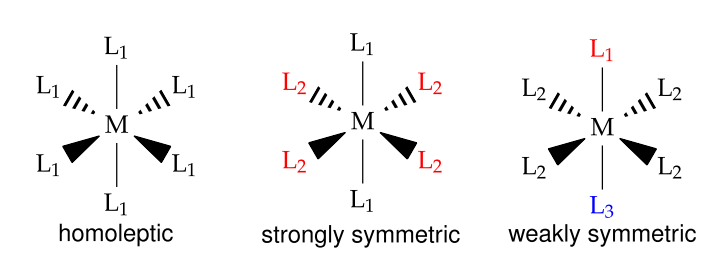
\includegraphics[width=0.8\textwidth]{img/symmetry_classes}
	\centering
	\caption{Examples for symmetry classes: A homoleptic complex with six times the same ligand, a strongly symmetric complex with the same ligand in axial and equatorial position, respectively, and a weakly symmetric ligand, which in addition also breaks the axial symmetry from the strongly symmetric complex.}
	\label{fig:sym-classes}
\end{figure}

To exemplify the scaling, we look at three different symmetry classes as shown in Figure \ref{fig:sym-classes}. Without loss of generality we chose the octahedral geometry for simplicity. The homoleptic case will result in 
\begin{equation}
	m \cdot l
\end{equation}
different complexes, where $m$ and $l$ are the number of available metal centers and ligands, respectively. For the strongly symmetric case, there will be
\begin{equation}
	m \cdot \frac{l!}{(l-2)!}
\end{equation}
distinguishable complexes, whereas in the weakly symmetric case we end up with 
\begin{equation}
	m \cdot  \frac{l!}{(l-3)! \cdot  2}
\end{equation}
complexes. Using four different metal centers and only 10 different ligands, we end up at 40, 360, and 1140 complexes. This exponential scaling prevents us from exhaustive analysis of the space. For lower symmetries, even enumeration becomes intractable. A complex with arbitrary ligands generates a data set with $4 \cdot 10^6$ complexes. 

\section{Spectrochemical Series}
\cite{tsuchida1938, ballhausen1963, griffith1957}


\bibliographystyle{achemso} % without .bst on windows/texmaker, with in kile/unix (?)
\bibliography{IECR_Paper} % without .bib
\end{document}